%%%%%%%%%%%%%%%%%%%%%%%%%%%%%%%%%%%%%%%%%%%%%%%%%%%%%%%%%%%%%%%%%%%%%%
% How to use writeLaTeX: 
%
% You edit the source code here on the left, and the preview on the
% right shows you the result within a few seconds.
%
% Bookmark this page and share the URL with your co-authors. They can
% edit at the same time!
%
% You can upload figures, bibliographies, custom classes and
% styles using the files menu.
%
% Modifyied by Prof. MSc. Daniel Menin Tortelli
% Computer Science - URICER - Brazil
%%%%%%%%%%%%%%%%%%%%%%%%%%%%%%%%%%%%%%%%%%%%%%%%%%%%%%%%%%%%%%%%%%%%%%

\documentclass[12pt]{article}


\usepackage{article-config/sbc-template}

\usepackage{graphicx,url}
\usepackage{float}

\usepackage[brazilian]{babel}   
\usepackage[T1]{fontenc} % Codificação para fontes com suporte a caracteres acentuados
\usepackage[utf8]{inputenc} % Codificação UTF-8 (necessário apenas para pdflatex)
\usepackage{multicol}
\usepackage{multirow}
\usepackage{graphicx,url}
\usepackage{amsmath,amssymb,amsfonts}
\usepackage{algorithmic}
\usepackage{textcomp}
\usepackage{url}
\usepackage{enumerate}
\usepackage{multirow}
\usepackage{soul}
\usepackage{verbatim}
\usepackage[table,xcdraw]{xcolor}
\usepackage[shortlabels]{enumitem}
\usepackage{scalefnt} % pacote para diminuir fonte das tabelas
\usepackage{comment} % pacote de comentarios
\usepackage{lscape}
\usepackage{fancyhdr}
\usepackage{article-config/pages-style}
\usepackage[super]{nth}
\usepackage[table]{xcolor}
\usepackage{pdflscape}
\usepackage{array}

\usepackage{listings}
\usepackage{xcolor}

\lstdefinestyle{mystyle}{
    backgroundcolor=\color{backcolour},   
    commentstyle=\color{codegreen},
    keywordstyle=\color{magenta},
    numberstyle=\tiny\color{codegray},
    stringstyle=\color{codepurple},
    basicstyle=\ttfamily\scriptsize,
    breakatwhitespace=false,         
    breaklines=true,                 
    captionpos=b,                    
    keepspaces=true,                 
    numbers=left,                    
    numbersep=5pt,                  
    showspaces=false,                
    showstringspaces=false,
    showtabs=false,                  
    tabsize=2
}
\lstset{style=mystyle}

%previne hifenização
\tolerance=1
\emergencystretch=\maxdimen
\hyphenpenalty=10000
\hbadness=10000

\sloppy


\curso{Ciência da Computação} % Preencha com o nome do curso
\local{URI Erechim/RS} % Local do evento
\ano{2025 } % Exemplo: 2025
\edicao{} % Exemplo: XXIII
\evento{\getedicao~Projeto de Conclusão de Curso \getano~-- \getlocal}


\title{Fuzzing Guiado por Contrato para APIs REST \\
\medskip
\small{
    \textit{Title: Contract-Guided Fuzzing for REST APIs}
  }
}

\author{Levi da Rosa Gomes (aluno)\inst{1}, Fábio Austrian Zanin (orientador)\inst{1}}

\address{
    Universidade Regional Integrada do Alto Uruguai e das Missões \\
    Departamento de Engenharias e Ciência da Computação\\
  Caixa Postal 743 -- 99.709-910 -- Erechim -- RS -- Brasil
\email{103495@uricer.edu.br, faz@uricer.edu.br}
}

\begin{document} 
\maketitle

\thispagestyle{plain}

\pagestyle{plain2}

\begin{abstract}
Divergences between REST API implementations and their OpenAPI contracts can
affect integration reliability and reveal robustness, conformance, and
access-control anomalies. This work presents a black-box, contract-guided
fuzzer and investigates the use of a fuzzy inference system to prioritize the
reported anomalies. The tool parses a supported subset of OpenAPI, generates
baseline and mutated inputs, executes HTTP requests, detects contractual
divergences, and preserves reproducible artifacts. Four APIs supported the
development and audit of the prioritization model; after its revision was
frozen, Meilisearch was used as an external holdout. The development pilot
executed 958 requests and produced 161 behavioral families. The initial model
reproduced the same categorical decisions as a status-only baseline, with
accuracy 0.298. On 122 supported holdout families, the revised model agreed
with a blind operational reference in 120 cases, compared with 4 for the
baseline. These partial results concern technical priority, not actual security
impact; the final experimental protocol remains subject to advisor review.
\end{abstract}

\keywords{REST APIs, OpenAPI, Fuzzing, Contract Testing, Fuzzy Logic.}
     
\begin{resumo}
Divergências entre implementações de APIs REST e seus contratos OpenAPI podem
afetar a confiabilidade das integrações e revelar anomalias de robustez,
conformidade e controle de acesso. Este trabalho apresenta um \textit{fuzzer}
de caixa-preta guiado por contrato e investiga o uso de um sistema de inferência
fuzzy para priorizar as anomalias reportadas. A ferramenta interpreta um
subconjunto de OpenAPI, gera entradas-base e mutações, executa requisições HTTP,
detecta divergências contratuais e preserva artefatos reproduzíveis. Quatro APIs
apoiaram o desenvolvimento e a auditoria do modelo de priorização; após o
congelamento de sua revisão, o Meilisearch foi utilizado como \textit{holdout}
externo. O piloto de desenvolvimento executou 958 requisições e produziu 161
famílias comportamentais. O modelo inicial reproduziu as mesmas decisões
categóricas de um \textit{baseline} baseado apenas em status, com acurácia
0,298. Nas 122 famílias sustentadas do \textit{holdout}, o modelo revisado
concordou com uma referência operacional cega em 120 casos, contra 4 do
\textit{baseline}. Esses resultados parciais tratam de prioridade técnica, não
de impacto real de segurança; o protocolo experimental final permanece sujeito
à avaliação do orientador.
\end{resumo}

\palavraschave{APIs REST, OpenAPI, Fuzzing, Teste de Contrato, Lógica Fuzzy.}

% CAPITULOS DO ARTIGO

% Estrutura do TCC
% TCC — Introdução
\section{Introdução}
APIs REST tornaram-se parte essencial da infraestrutura de sistemas modernos, conectando serviços, aplicações web e dispositivos móveis \cite{arcuri2026fuzzingrestapisindustry}. Nesse cenário, falhas de robustez e inconsistências entre o comportamento da API e o contrato publicado impactam diretamente a confiabilidade de integrações e o custo de manutenção. Embora testes funcionais tradicionais sejam eficazes para validar cenários felizes (\textit{happy path}), eles frequentemente deixam de exercitar valores-limite, formatos inválidos e combinações pouco usuais de parâmetros, que são justamente as situações em que falhas sutis tendem a se manifestar.

O uso de contratos formais, como a especificação OpenAPI (versões 3.0 e 3.1), viabiliza uma abordagem "guiada por contrato" para a geração de casos de teste: em vez de produzir entradas aleatórias, o processo explora estruturas, tipos e restrições descritas no \textit{schema} para produzir mutações \emph{válidas e inválidas} de forma sistemática. Essa estratégia aumenta a probabilidade de revelar respostas inesperadas (por exemplo, códigos 5xx, mensagens de erro inconsistentes ou divergências estruturais entre a resposta e o contrato) sem exigir acesso ao código-fonte nem instrumentação interna da aplicação, isto é, em um contexto \emph{black-box} \cite{meyer1992designbycontract}.

Este trabalho propõe o desenvolvimento e a avaliação de uma ferramenta de \emph{fuzzing} automatizado para APIs REST baseada em contratos OpenAPI. A ferramenta implementa: (i) um \textit{parser} que converte um subconjunto da especificação em um modelo interno; (ii) um motor que produz entradas-base e aplica mutações orientadas por tipos e por parte das restrições representadas; (iii) um plano de execução e um \textit{runner} de requisições com controle de concorrência; e (iv) um analisador que registra evidências e identifica divergências em relação ao contrato interpretado. A avaliação caracteriza os achados produzidos em APIs distintas, sua reprodução entre campanhas e a utilidade do mecanismo de priorização.

Além da identificação de divergências contratuais, a ferramenta utiliza um sistema de inferência fuzzy do tipo Mamdani para atribuir um escore contínuo aos achados reportados. Esse componente não confirma automaticamente defeitos ou vulnerabilidades: sua função é apoiar a priorização da inspeção humana a partir de sinais observáveis da execução. Nesse contexto, a pesquisa investiga quais tipos de achado o \textit{fuzzer} produz em APIs distintas, em que medida esses achados são reproduzíveis e quão coerente é o ordenamento de severidade em relação a critérios humanos definidos independentemente do escore.

O escopo delimita-se a APIs REST descritas em OpenAPI, não abrangendo cenários dependentes de sequenciamento complexo de requisições ou manutenção de estado entre chamadas, autenticação avançada (por exemplo, fluxos completos de OAuth2) nem avaliação de carga ou desempenho. A ferramenta gera saídas estruturadas compatíveis com automação, mas a integração completa e a efetividade em fluxos de CI/CD não constituem objetos centrais da avaliação.

O restante deste artigo está organizado da seguinte forma. A Seção~\ref{sec:fundamentacao} apresenta os conceitos de OpenAPI, \textit{fuzzing} de APIs e lógica fuzzy necessários à compreensão do trabalho. A Seção~\ref{sec:relacionados} discute ferramentas e pesquisas relacionadas e posiciona a proposta. A Seção~\ref{sec:metodologia} descreve o delineamento e o protocolo de avaliação, enquanto a Seção~\ref{sec:desenvolvimento} detalha a arquitetura e as decisões da implementação. A Seção~\ref{sec:resultados} apresenta e discute os resultados experimentais. Por fim, a Seção~\ref{sec:conclusoes} sintetiza as contribuições, limitações e possibilidades de continuidade.

% TCC — Fundamentação Teórica
\section{Fundamentação Teórica}\label{sec:fundamentacao}

Esta seção delimita os conceitos necessários para compreender a geração de
testes guiada por contratos e o mecanismo de priorização. A versão definitiva
incorporará as fontes primárias já mapeadas na revisão bibliográfica.

\subsection{APIs REST e Especificação OpenAPI}

Neste trabalho, o documento OpenAPI exerce dois papéis. Primeiro, fornece
estrutura para gerar operações, parâmetros e corpos de requisição. Segundo,
atua como oráculo parcial ao descrever status e schemas esperados nas respostas.
Esse oráculo é incompleto: uma API pode aplicar regras de negócio ausentes do
contrato, e o contrato também pode divergir da implementação sem que exista
falha de segurança.

\textit{[Sketch para orientação: incorporar definições e fontes primárias sobre
REST, OpenAPI e contrato como oráculo parcial.]}

\subsection{Teste Negativo e Fuzzing}

Teste negativo exercita entradas inválidas, limites e combinações adversas para
observar se o sistema rejeita dados de forma controlada. O \textit{fuzzing}
pode ser geracional, quando produz casos a partir de um modelo, ou mutacional,
quando transforma entradas existentes. A ferramenta combina as duas ideias:
gera um valor-base do contrato e aplica operadores tipados. Diferentemente de
fuzzers guiados por cobertura, a observação permanece \textit{black-box}.

\textit{[Sketch para orientação: incorporar fontes primárias sobre teste
negativo, robustez e fuzzing geracional/mutacional.]}

\subsection{Fuzzing de APIs REST Guiado por Contrato}

APIs introduzem desafios de dados estruturados, autenticação, dependências
entre recursos, estado e serialização. OpenAPI permite orientar entradas e
comparar respostas, mas não resolve automaticamente essas dependências nem
garante a completude do oráculo. Por isso, rejeições seguras não documentadas,
aceitações indevidas, erros de servidor e divergências de schema precisam ser
descritos separadamente.

\textit{[Sketch para orientação: consolidar aqui as fontes de fuzzing de APIs e
os limites conhecidos de abordagens exclusivamente black-box.]}

\subsection{Lógica Fuzzy e Prioridade Técnica}

Um sistema Mamdani representa conceitos graduais por funções de pertinência,
combina antecedentes em regras linguísticas, agrega suas ativações e produz um
valor contínuo por desfuzzificação. Essa estrutura favorece uma priorização
interpretável, pois permite preservar entradas, pertinências e regras ativadas.

Neste trabalho, a saída representa prioridade técnica da anomalia. Ela não
confirma vulnerabilidade, explorabilidade, impacto de negócio ou urgência real
de correção. O modelo revisado utiliza contradição comportamental, força da
evidência e exposição de controle de acesso como antecedentes. A detecção
contratual ocorre antes da priorização e constitui uma responsabilidade
conceitualmente distinta.

\textit{[Sketch para orientação: incorporar fundamentos de conjuntos fuzzy,
inferência Mamdani e priorização, distinguindo parâmetros heurísticos de
parâmetros apoiados pela literatura.]}

% TCC — Trabalhos Relacionados
\section{Trabalhos Relacionados}\label{sec:relacionados}

Esta seção posiciona o projeto diante de ferramentas que também testam APIs
REST a partir de contratos. A comparação é bibliográfica e não representa uma
execução conjunta das ferramentas. O objetivo é identificar capacidades e
limites relevantes para o recorte do TCC, sem produzir um ranking entre
soluções com objetivos diferentes.

Os critérios usados são: fonte do modelo de entrada; modo de acesso à
aplicação; estratégia de geração; tratamento de estado e dependências; forma
do oráculo; possibilidade de reproduzir os resultados; e organização ou
priorização dos achados.

\subsection{Ferramentas selecionadas}

\paragraph{Schemathesis.}
Schemathesis deriva testes baseados em propriedades a partir de schemas de
APIs. A geração usa tipos e restrições do contrato e aplica verificações
semânticas às respostas observadas \cite{hatfielddodds2022schemathesis}. A
abordagem é black-box e inclui mecanismos para reduzir e reproduzir casos que
falham. Ela é a ferramenta mais próxima do projeto no uso direto do contrato
para gerar entradas e verificar propriedades, mas seu foco é o teste baseado
em propriedades, não a atribuição de uma prioridade fuzzy aos achados.

\paragraph{RESTler.}
RESTler compila uma especificação Swagger/OpenAPI em uma gramática e infere
dependências produtor--consumidor entre operações. Com isso, gera sequências
stateful que criam o estado necessário antes de exercitar parâmetros
\cite{atlidakis2019restler}. O trabalho também descreve checkers e mecanismos
de agrupamento de bugs. RESTler é uma referência para dependências entre
operações; o fuzzer deste TCC cobre esse aspecto apenas parcialmente e não
pretende oferecer a mesma exploração stateful.

\paragraph{RESTest.}
RESTest realiza teste black-box orientado por OpenAPI e combina geração
aleatória com restrições adicionais. O framework contempla casos nominais e
de falha e associa oráculos aos casos gerados \cite{martinlopez2020restest}.
Essa abordagem ajuda a separar o uso do contrato da implementação de um
oráculo, mas depende do modelo e das restrições disponíveis. O projeto se
aproxima no teste negativo e se diferencia pelo catálogo de mutações e pela
priorização posterior dos achados.

\paragraph{RestTestGen.}
RestTestGen apresenta uma arquitetura extensível para teste black-box, com
parser OpenAPI, provedores de valores, geradores, mutadores, executor e
oráculos \cite{corradini2022resttestgen}. A decomposição é útil para comparar
componentes do pipeline e para discutir reprodução dos artefatos. O trabalho
não define um classificador fuzzy de prioridade; essa é uma parte específica
da proposta deste TCC.

\subsection{Síntese da comparação}

\begin{table}[ht]
\centering
\scalefont{0.82}
\caption{Posicionamento bibliográfico das ferramentas selecionadas}
\label{tab:ferramentas-relacionadas}
\begin{tabular}{|p{2.3cm}|p{2.3cm}|p{1.7cm}|p{2.3cm}|p{2.4cm}|p{2.4cm}|}
\hline
\textbf{Ferramenta} & \textbf{Entrada e geração} & \textbf{Acesso} & \textbf{Estado} & \textbf{Oráculo} & \textbf{Prioridade} \\ \hline
Schemathesis & Schema + property-based & Black-box & Fluxos conforme configuração & Checks e propriedades & Não identificada na fonte-base \\ \hline
RESTler & Gramática + sequências & Black-box & Stateful, produtor--consumidor & Checkers e respostas & Não é foco \\ \hline
RESTest & OpenAPI + restrições & Black-box & Dependente do modelo & Oráculos dos casos & Não é foco \\ \hline
RestTestGen & Framework modular + mutadores & Black-box & Extensível & Oráculos extensíveis & Não identificada \\ \hline
Projeto & OpenAPI + mutações tipadas & Black-box & Parcial & Contrato e detectores & FIS Mamdani pós-execução \\ \hline
\end{tabular}
\end{table}

As quatro ferramentas mostram que “usar OpenAPI” não define uma única técnica.
Elas diferem na maneira de gerar dados, montar sequências, lidar com estado e
interpretar respostas. Os trabalhos de revisão também apontam dificuldades
recorrentes: dependências entre operações, autenticação, dados realistas e
reprodução das execuções. Esses fatores precisam ser controlados ou registrados
para que duas campanhas possam ser comparadas \cite{golmohammadi2023rest,zhang2023openproblems}.

O projeto não reivindica novidade por gerar casos a partir de OpenAPI, testar
entradas negativas ou verificar status e schema. A proposta investigada é mais
específica: combinar mutações estruturadas, evidências reproduzíveis e um
sistema fuzzy que ordena os achados depois da execução. A metodologia avalia
essa combinação no corpus definido; não há comparação experimental suficiente
para afirmar superioridade sobre as ferramentas relacionadas.

\subsection{Critério para eventual comparação experimental}

Schemathesis é a candidata mais próxima caso o orientador considere útil uma
comparação prática. Para ser válida, ela teria de usar os mesmos contratos,
alvos, número de campanhas, condições de reset e orçamento aproximado. As
métricas deveriam permanecer limitadas às definidas no TCC: requisições
concluídas, divergências observadas, famílias deduplicadas, estabilidade e
reprodução dos artefatos. Cobertura interna, qualidade de implementação ou
superioridade de uma ferramenta não seriam inferidas sem um protocolo próprio.

Por ora, RESTler, RESTest e RestTestGen cumprem papel de referências
arquiteturais e metodológicas. EvoMaster e Dredd permanecem registrados no
material de apoio, mas não entram nesta comparação até que sua utilidade e a
fonte primária adequada sejam confirmadas.

% TCC — Metodologia
\section{Metodologia}\label{sec:metodologia}

Esta pesquisa é aplicada e experimental e avalia um \textit{fuzzer}
\textit{black-box} orientado por contratos OpenAPI. A investigação considera
três perguntas complementares: quais divergências técnicas são observadas em
APIs distintas, com que estabilidade os comportamentos reaparecem em campanhas
repetidas e se a priorização ajuda a organizar os achados para triagem. Neste estudo, o
sistema de inferência fuzzy (FIS) atribui uma prioridade técnica a cada
anomalia observada. A pontuação não representa explorabilidade, impacto real
nem gravidade de segurança demonstrada.

As três formulações abaixo são mantidas provisoriamente para escolher a
pergunta que melhor representa o trabalho:

\begin{enumerate}
    \item \textit{Como um pipeline black-box orientado por OpenAPI pode
    produzir evidências reprodutíveis e priorizadas para a triagem de
    divergências em APIs REST durante ciclos de integração contínua?}
    \item \textit{De que forma um fuzzer black-box orientado por OpenAPI pode
    transformar divergências observadas em evidências reproduzíveis,
    deduplicadas e priorizadas para a triagem de APIs REST em ciclos de
    integração contínua?}
    \item \textit{Quais evidências de execução, estabilidade e prioridade um
    pipeline black-box orientado por OpenAPI produz ao testar APIs REST, e
    quais condições determinam sua utilidade para triagem em ciclos de
    integração contínua?}
\end{enumerate}

Nas três versões, integração contínua delimita o contexto de uso. O trabalho
não implementa workflow, plugin, quality gate ou outra integração específica
com uma esteira.

\subsection{Desenho do Estudo e Papel das Aplicações}

VAmPI, Spring Petclinic REST, crAPI e RealWorld formaram o conjunto usado para
desenvolver e caracterizar o fuzzer. Os resultados dessas aplicações permitiram
auditar a configuração inicial do mecanismo de priorização e formular sua
revisão. O Meilisearch v1.45.1 foi executado somente depois dessa revisão, como
uma aplicação externa de confirmação, sem participar do ajuste das novas regras.

As aplicações foram executadas localmente em versões fixadas e reiniciáveis.
Contratos, imagens, configuração do fuzzer e procedimentos de inicialização
foram registrados para separar mudanças do objeto avaliado de variações do
ambiente.

A coleta final terá cinco campanhas independentes para cada aplicação. Antes de
cada campanha, a aplicação e os dados necessários serão reiniciados para que o
resultado não dependa do estado deixado pela execução anterior. As quatro APIs
usadas no desenvolvimento continuarão identificadas como conjunto de pilotos. O
Meilisearch será analisado no mesmo conjunto de campanhas, mas manterá o papel
separado de aplicação externa ao desenvolvimento do FIS.

O Meilisearch já possui cinco campanhas completas. Elas serão reaproveitadas
somente se a conferência dos manifestos (arquivos de registro da execução)
confirmar a mesma revisão do fuzzer,
contrato, configuração, procedimento de reset e conjunto de artefatos exigidos
para a coleta. Se algum desses elementos não puder ser comprovado, as
campanhas serão repetidas. A data não precisa ser igual à das demais APIs; o
que precisa ser igual é o protocolo registrado.

A repetição não existe para fazer o fuzzer sortear casos diferentes. Com o mesmo
contrato, revisão e configuração, o plano de requisições tende a ser o mesmo.
Ela verifica se as respostas, os achados e as assinaturas se mantêm depois do
reset. Essa distinção é necessária porque a execução ainda pode variar: alguns
runners geram credenciais automaticamente, e o estado da aplicação, o tempo de
resposta ou uma falha transitória podem mudar entre campanhas.

\subsection{Geração dos Testes e Níveis de Mutação}

A geração começa com um caso compatível com as informações interpretadas do
contrato. A partir dele, o motor aplica operadores tipados sobre parâmetros e
corpos. Três níveis organizam a exploração:

\begin{itemize}
    \item \textbf{Nível 0 (L0) --- caso-base:} executa a entrada gerada para
    satisfazer o contrato e estabelece a referência nominal da operação;
    \item \textbf{Nível 1 (L1) --- mutação isolada:} aplica uma alteração por
    caso, permitindo relacionar a resposta com um operador específico;
    \item \textbf{Nível 2 (L2) --- mutações combinadas:} combina duas alterações
    compatíveis para explorar interações, preservando orçamento próprio e os
    casos isolados de L1.
\end{itemize}

Essa progressão distingue comportamento nominal, efeito individual e interação
entre mutações. O plano também inclui, quando habilitados, testes de operações
protegidas sem credencial ou com credencial inválida. Limites de casos,
concorrência, atraso e timeout são registrados como parte da configuração.

\subsection{Protocolo Experimental e Estratégia de Avaliação}

Cada campanha segue o fluxo contrato, plano, execução, análise e
pós-processamento. Um manifesto registra identificador do experimento, API,
repetição, revisão do código, estado Git, hashes, ambiente, configuração,
horários e contagens. O plano e os resultados são correlacionados por
\texttt{case\_id}; campanhas incompletas ou inválidas devem permanecer
identificáveis, em vez de desaparecer das evidências.

As campanhas definitivas usam a configuração já exercitada nos pilotos. O
runner percorre todas as operações suportadas pelo módulo que interpreta o
contrato e executa os níveis L0, L1 e L2. O limite configurado é de 20 casos de
mutação isolada por payload no L1 e de 10 pares compatíveis no L2. Esses limites
são fixos; a quantidade efetiva pode ser menor quando o contrato oferece menos
parâmetros, esquemas ou combinações aplicáveis. A concorrência fica em 1, o
intervalo entre requisições em 250 ms e o timeout em 10 s. A autenticação
automática é usada somente nos alvos em que o runner consegue configurá-la de
forma reproduzível.

Aqui, contrato significa o arquivo OpenAPI de cada alvo. Ele descreve as
operações, caminhos, parâmetros, corpos e respostas que o runner consegue
interpretar. Por isso, contratos diferentes geram quantidades diferentes de
casos e de requisições; não se espera que todas as APIs produzam o mesmo total.
Cada manifesto registra o número planejado e o número executado, além da
configuração usada, para que a comparação aplique a mesma regra a contratos de
tamanhos distintos.

Antes da execução, o healthcheck do alvo precisa passar. Durante a campanha,
``acessível'' significa que o processo continua disponível o suficiente para o
runner concluir o plano. Uma resposta 4xx ou 5xx de uma operação é uma
observação do teste e não invalida, por si só, a campanha. Já falha de
inicialização, falha no reset, encerramento do processo ou interrupção que deixe
requisições sem resultado impedem a interpretação completa da execução.

Uma campanha válida tem o plano completo, um resultado relacionável a cada
\texttt{case\_id}, artefatos legíveis e registro da versão do alvo, da revisão do
fuzzer e da configuração. Quando isso não ocorre, a campanha recebe status
inválido e a justificativa fica junto dos seus logs e artefatos; ela não entra no
agregado válido e não é apagada. Se a causa puder ser corrigida, uma nova
campanha é executada com o mesmo protocolo. A execução original continua
preservada como evidência da falha, e a nova execução recebe seu próprio
identificador.

\begin{figure}[H]
    \centering
    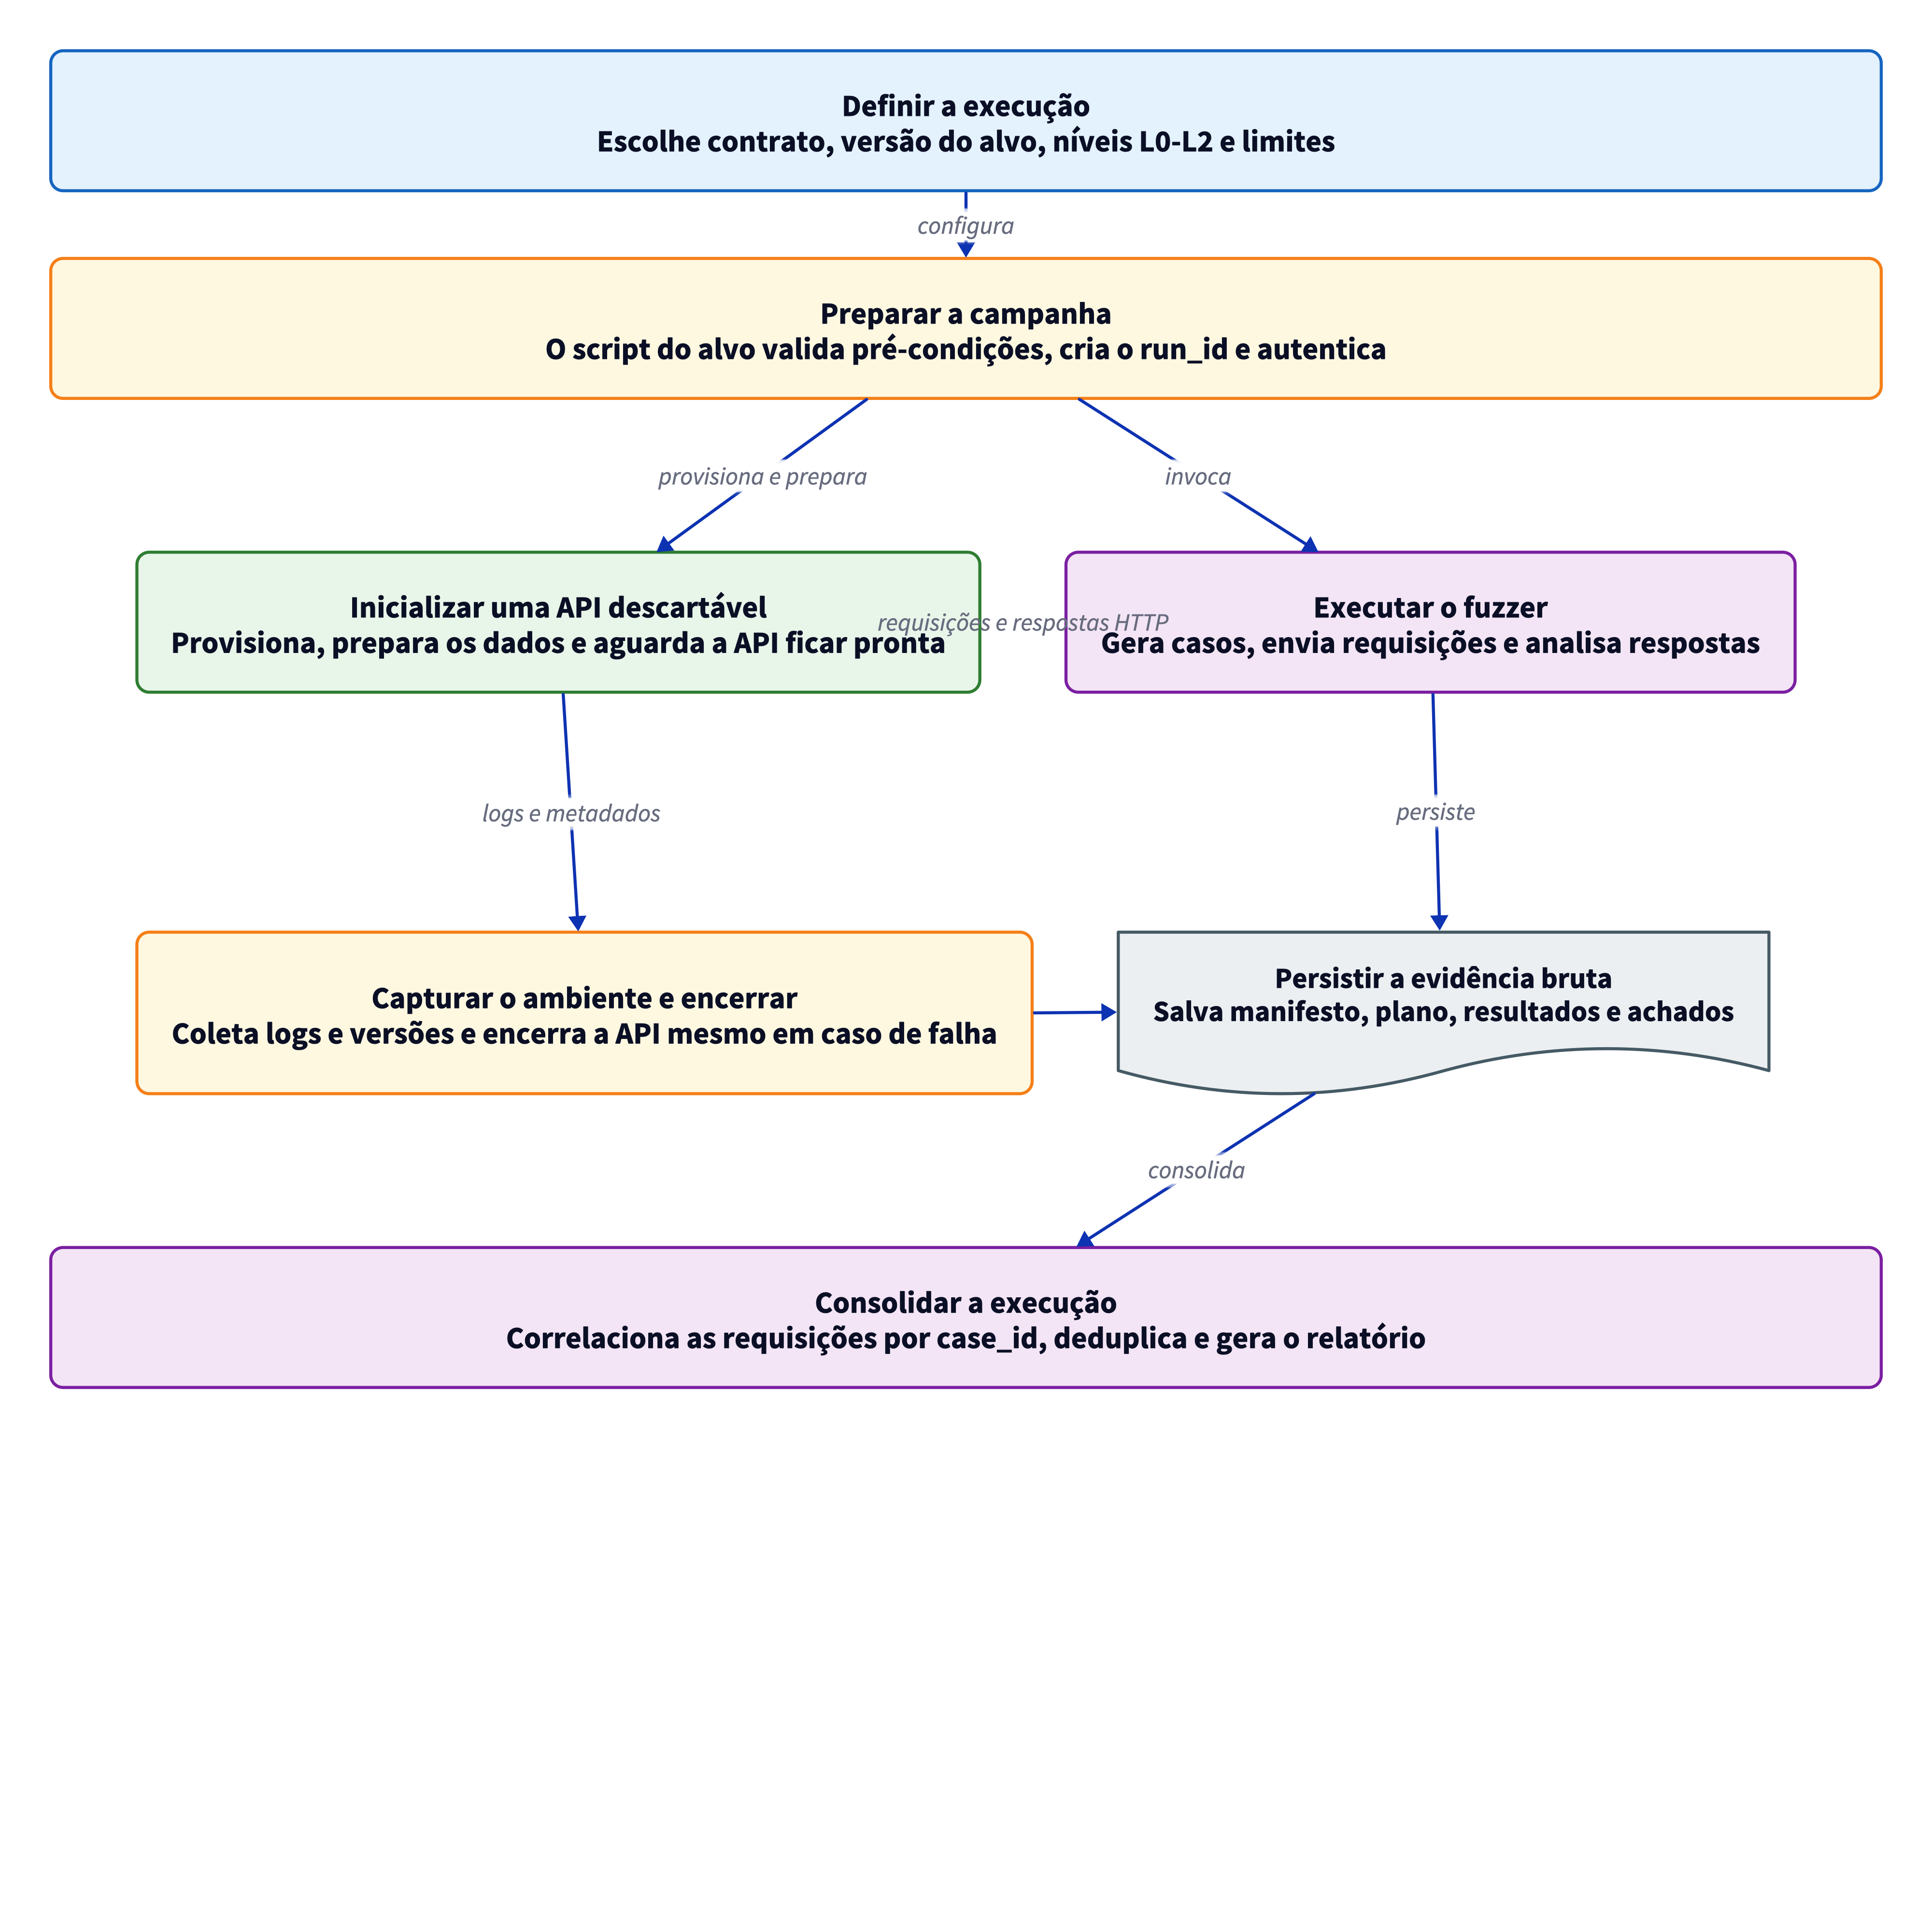
\includegraphics[width=0.90\linewidth]{Diagrams/experimental-architecture.png}
    \caption{Ciclo de uma execução experimental isolada. O script específico
    prepara o alvo descartável e invoca o fuzzer. A ligação HTTP representa a
    troca de requisições e respostas; a evidência é completada com a
    proveniência do alvo antes da deduplicação e consolidação.}
    \label{fig:ciclo-experimental}
\end{figure}

Para acompanhar uma execução sem misturar coisas diferentes, o estudo separa
cinco unidades:

\begin{itemize}
    \item uma \textbf{requisição}, que é um caso enviado à API;
    \item um \textbf{achado}, que é a divergência observada nessa requisição;
    \item uma \textbf{assinatura}, isto é, um identificador que agrupa
    observações equivalentes por aplicação, operação, classificação, status e
    resposta normalizada;
    \item uma \textbf{campanha}, que é uma execução completa contra uma API;
    \item uma \textbf{família de comportamento}, que reúne assinaturas que
    descrevem o mesmo comportamento factual por endpoint e tipo de divergência.
\end{itemize}

Essa separação evita contar várias mutações que produziram a mesma resposta
como falhas diferentes. Ela também não afirma que cada grupo corresponde a uma
causa raiz no código da aplicação.

Para comparar a prioridade atribuída pelo FIS, foi construída uma referência
independente do seu resultado. Cada família foi apresentada com o contrato, a
requisição, a resposta e a repetição observada, mas sem mostrar a classificação
do analisador nem a prioridade calculada pelo FIS. Três avaliações independentes
aplicaram a mesma rubrica de LOW, MEDIUM e HIGH. Quando não houve maioria, uma
quarta avaliação decidiu o caso sem acesso às avaliações anteriores ou ao FIS.
Essa referência serve para a comparação operacional; não é uma avaliação de
especialistas humanos e não confirma vulnerabilidades.

O FIS é comparado com uma regra mais simples, que usa apenas o desvio do status
HTTP. As duas abordagens recebem as mesmas famílias como entrada. A análise
registra a proporção de classificações iguais, o desempenho por classe (LOW,
MEDIUM e HIGH), a distância entre erros de prioridade e a correlação entre o
ranking produzido e a referência. A estabilidade é medida pela presença de
uma mesma assinatura nas cinco campanhas, sem um replay adicional de cada
requisição. Uma assinatura é considerada estável quando aparece em pelo menos
quatro campanhas sob a mesma configuração.

\subsection{Limitações e Ameaças à Interpretação}

As limitações abaixo explicam o que pode influenciar os resultados e até onde
eles podem ser generalizados.

\paragraph{O que é medido.}
O contrato OpenAPI funciona como uma referência parcial: ele descreve o
comportamento esperado, mas pode omitir regras existentes na implementação. O
fuzzer também interpreta apenas o subconjunto de OpenAPI que suporta. Por isso,
uma divergência encontrada é um comportamento que merece inspeção, não uma
prova automática de defeito ou vulnerabilidade. O FIS ordena a prioridade
técnica desse comportamento; sua pontuação não estima impacto real, explorabilidade
ou gravidade de segurança. A assinatura agrupa respostas equivalentes, mas não
identifica a causa no código.

\paragraph{Condições da execução.}
Estado residual, ordem das requisições, latência da máquina e falhas internas da
aplicação podem mudar o resultado de uma campanha. O reset entre campanhas,
concorrência 1, atraso fixo e manifestos reduzem essas diferenças. Ainda assim,
não é possível garantir que toda variação do ambiente tenha sido eliminada.

\paragraph{Alcance das aplicações.}
O estudo usa cinco aplicações: quatro participaram do desenvolvimento e dos
pilotos, e o Meilisearch foi mantido como aplicação externa para confirmar a
priorização. Esse desenho permite testar o modelo fora do conjunto de
desenvolvimento que o originou,
mas não representa a variedade de todas as APIs REST. As conclusões ficam
limitadas às aplicações, contratos, versões e configurações avaliados.

\paragraph{Força das conclusões.}
O número de famílias e a distribuição entre LOW, MEDIUM e HIGH limitam algumas
métricas. A referência de prioridade foi produzida às cegas segundo uma rubrica,
com avaliações independentes, mas não por especialistas humanos. O trabalho
também não mede cobertura de código, não implementa integração com CI ou
quality gate e não confirma vulnerabilidades automaticamente. Essas questões
ficam fora do que os resultados podem afirmar.

% TCC — Desenvolvimento
\section{Desenvolvimento da Ferramenta}\label{sec:desenvolvimento}

\subsection{Arquitetura e Fluxo Operacional}

O OpenAPI Contract Fuzzer foi implementado em Python como um pipeline modular.
O contrato é convertido em um modelo interno; esse modelo orienta a geração de
valores-base e mutações; um plano materializa as requisições; o executor envia
as chamadas à API; e o analisador confronta as respostas com o contrato antes
de encaminhar os resultados reportáveis ao sistema fuzzy e ao gerador de
relatórios.

% TODO(TCC): inserir diagrama editável:
% OpenAPI -> Parser -> Modelo -> Geração/Mutação -> Plano/Runner -> API
% -> Analisador Contratual -> FIS -> Relatório.

\subsection{Interpretação do Contrato e Geração de Entradas}

O parser atual aceita documentos YAML ou JSON e representa operações,
parâmetros, corpos JSON, respostas e mecanismos de segurança dentro de um
subconjunto de OpenAPI. A partir do modelo, o gerador produz valores-base e o
motor aplica operações de substituição ou remoção sobre tipos primitivos,
objetos e arrays.

O suporte não é integral: referências e composições de schema, diferentes
\textit{media types} e parte das regras de serialização ainda não são
interpretados. Além disso, o catálogo existente é predominantemente orientado
por tipos. O texto e a avaliação deverão distinguir restrições efetivamente
usadas de capacidades ainda não implementadas.

\subsection{Planejamento e Execução}

O plano de execução associa operação, caminho resolvido, corpo e cabeçalhos.
Autenticação pode ser fornecida por configuração ou obtida por um procedimento
automático baseado no contrato. A execução utiliza um cliente HTTP assíncrono e
um semáforo para limitar a concorrência, preservando a ordem lógica entre plano
e resultados.

\subsection{Detecção de Divergências}

O analisador identifica respostas sem status, erros de servidor, status não
documentados, incompatibilidades de schema e aceitação de entradas mutadas.
Uma rejeição 4xx documentada e compatível com o schema é comportamento esperado
e não deve ser contabilizada como anomalia candidata.

Um achado reportado não equivale automaticamente a defeito ou vulnerabilidade.
A confirmação exige reprodução e inspeção das condições do contrato, da entrada
e do ambiente.

\subsection{Priorização por Lógica Fuzzy}

Após a classificação contratual, o sistema Mamdani combina desvio de status,
tempo de resposta e tamanho da resposta para produzir um escore contínuo,
posteriormente dividido nas faixas LOW, MEDIUM e HIGH. As funções de
pertinência, regras e limiares atuais são escolhas heurísticas do autor; sua
coerência constitui objeto da avaliação, não uma propriedade presumida.

\subsection{Artefatos e Rastreabilidade}

Cada campanha produz plano, resultados brutos, achados estruturados e relatório
em Markdown. Antes da coleta definitiva, os artefatos deverão incluir
identificador de caso, mutação aplicada, versão do contrato, configuração e
seed, permitindo deduplicação, reexecução e rastreabilidade dos números
apresentados no artigo.

% TCC — Resultados e Discussão
\section{Resultados e Discussão}\label{sec:resultados}

Esta seção registra inicialmente os resultados do piloto usados para auditar e
revisar o mecanismo de priorização. Os números ainda não constituem a avaliação
externa final do FIS revisado. Resultados negativos e casos que contradigam as
hipóteses são preservados porque explicam as decisões posteriores do projeto.

\subsection{Caracterização do Piloto}

Foram executadas campanhas de nível 2 contra VAmPI, Spring Petclinic REST,
crAPI e RealWorld. No conjunto canônico, 958 requisições planejadas foram
executadas, das quais 284 continham combinações de duas mutações. A
deduplicação estrita produziu 265 assinaturas: 7 na VAmPI, 47 na Petclinic, 198
na crAPI e 13 na RealWorld. Para a avaliação de prioridade, essas assinaturas
foram reunidas em 161 famílias de comportamento.

O nível 2 ampliou a variedade das manifestações observadas, especialmente na
crAPI, onde 37 assinaturas novas envolveram combinações L2. No entanto, o
piloto não produziu uma nova família de anomalia de prioridade alta exclusiva
desse nível. O resultado não torna o L2 irrelevante: divergências de contrato,
respostas combinadas e variações de robustez também fazem parte do objeto de
estudo, mesmo quando não indicam vulnerabilidade grave.

\subsection{Construção da Referência Cega}

Três julgadores agentes avaliaram as 161 famílias sem acesso ao rótulo do
analisador ou aos resultados do FIS. Houve concordância exata sobre validade em
144 famílias (89,4\%). As mesmas 144 foram consideradas suportadas pelos três
julgadores, com concordância exata de prioridade em 136 casos (94,4\%). Sete
casos sem maioria de prioridade foram submetidos a um quarto julgador. A
referência final manteve todas as famílias como suportadas e distribuiu-as em
99 LOW, 59 MEDIUM e 3 HIGH.

As três famílias HIGH corresponderam a duas falhas 500 repetidas em baselines
válidos da Petclinic e a uma operação autenticada da crAPI que aceitou
credencial ausente e retornou conteúdo funcional. A referência é descrita como
operacional e assistida por agentes, não como verdade humana absoluta.

\subsection{Avaliação da Priorização Fuzzy}

A auditoria do FIS v2 mostrou que o status HTTP dominava a decisão. A ablação
do tempo e a ablação do sinal de tamanho não alteraram a faixa de nenhuma das
161 famílias. O v2 e o baseline baseado apenas em status obtiveram a mesma
acurácia, 0,298, o mesmo macro-F1, 0,254, e o mesmo erro ordinal médio, 0,702.
O v2 apresentou correlação de Spearman de 0,710 com a referência.

A matriz de confusão explicou a baixa acurácia: 67 famílias LOW foram elevadas
a MEDIUM e 43 famílias MEDIUM foram elevadas a HIGH. O modelo
superpriorizava rejeições seguras, status 4xx não documentados e falhas 5xx
localizadas. Em particular, uma resposta 4xx não documentada pode representar
contract drift e ainda assim constituir rejeição segura da entrada exercitada;
as duas propriedades precisam ser preservadas sem receber automaticamente a
mesma prioridade de uma operação válida indisponível.

Esse resultado motivou o FIS v3. Seus antecedentes são contradição
comportamental, força da evidência e exposição de controle de acesso. Tempo e
tamanho deixaram de integrar o núcleo da decisão. Repetição após deduplicação
fortalece a evidência de falhas de servidor; credencial ausente e inválida são
tratadas separadamente; e a conformidade da resposta é recalculada contra o
contrato, sem usar o rótulo final do analisador como antecedente.

Aplicado às mesmas 161 famílias de desenvolvimento, o código do v3 reproduziu
todas as faixas da referência, com macro-F1 1,000 e erro ordinal zero. Esse
resultado comprova que a implementação expressa a rubrica formulada, mas não
estima generalização: as regras foram definidas depois da análise desta
amostra. Uma quinta API ou um conjunto futuro congelado antes da rotulagem é
necessário para a avaliação confirmatória.

\subsection{Casos Representativos e Falsos Positivos}

Os desacordos do v2 mostraram três padrões importantes. Primeiro, rejeições
404 de identificadores gerados não comprovam falha da operação e tendem a LOW.
Segundo, um baseline POST cujo corpo satisfaz o schema OpenAPI, mas recebe 400
por restrições não declaradas pelo contrato, evidencia contract drift de
entrada e tende a MEDIUM. Terceiro, um erro 500 isolado possui evidência mais
fraca que o mesmo comportamento repetido em diferentes casos; por isso, a
recorrência atua como modificador de prioridade no v3.

\subsection{Discussão Geral}

O principal resultado do piloto não é que o FIS v2 tenha superado um baseline,
mas que a instrumentação permitiu demonstrar por que ele não o superava. A
revisão substituiu sinais fáceis de medir, porém pouco discriminativos, por
fatos mais próximos do construto. A contribuição deve ser apresentada como um
processo auditável de priorização de anomalias técnicas, incluindo contract
drift e robustez, e não como estimador de impacto real ou gravidade de
segurança.

Permanecem como ameaças a quantidade de APIs, a dependência do OpenAPI como
oráculo parcial, a correlação entre julgadores agentes e o ajuste do v3 no
mesmo conjunto usado para diagnosticar o v2. As campanhas definitivas devem
congelar código, regras e protocolo antes da coleta confirmatória.

% TCC — Conclusão
\section{Conclusão}\label{sec:conclusoes}

Este trabalho investigou quais contribuições e limitações a combinação de
\textit{fuzzing} \textit{black-box} orientado por OpenAPI, deduplicação e
priorização \textit{fuzzy} apresenta para a triagem de divergências em APIs
REST. Para isso, foi implementado um fluxo que interpreta um subconjunto de
OpenAPI, gera casos-base e mutações, executa as requisições, identifica
divergências, agrupa observações equivalentes, atribui prioridade técnica e
preserva os artefatos de cada campanha.

Nas três dimensões avaliadas, os resultados indicam:

\begin{itemize}
    \item \textbf{execução e completude:} as 25 campanhas da coleta final
    concluíram as 7.175 requisições planejadas, e as contagens do artigo podem
    ser rastreadas até os planos, as respostas e os achados publicados;
    \item \textbf{estabilidade:} 441 dos 570 IDs semânticos reapareceram nas
    cinco repetições da respectiva API e 453 em pelo menos quatro. A presença
    foi completa no Petclinic REST e no Meilisearch; em VAmPI e RealWorld, a
    variação veio de dados gerados em cada campanha, e a crAPI concentrou a
    maior parte dos IDs observados uma única vez;
    \item \textbf{deduplicação e prioridade:} o agrupamento reduziu 4.000
    achados brutos a 2.460 assinaturas estritas (38,5\%). Na Etapa 1, o FIS
    revisado concordou com a referência cega em 120 de 122 famílias do
    Meilisearch, contra 4 da linha de base baseada somente no status.
\end{itemize}

A principal contribuição é um processo rastreável que transforma um contrato
OpenAPI em evidências organizadas para triagem de \textit{contract drift},
incompatibilidades funcionais, problemas de robustez e indícios de controle de
acesso, com uma prioridade cujos critérios podem ser auditados. Os resultados
não confirmam vulnerabilidades nem estimam impacto real. As conclusões são
limitadas pelo número de aplicações, pelos recortes dos contratos, pelo OpenAPI
como oráculo parcial e por uma referência de prioridade produzida por um modelo
de linguagem, sem casos \texttt{HIGH} no Meilisearch. Na coleta final, os
escores têm interpretação descritiva.

Como trabalhos futuros, ficam a ampliação das aplicações e dos recursos de
OpenAPI suportados, a resolução de dependências entre operações, a avaliação da
triagem por especialistas humanos, a integração com uma esteira de integração
contínua e a comparação com outras ferramentas sob um mesmo protocolo.


\section{Referências}

\bibliographystyle{article-config/sbc}
\renewcommand{\refname}{}
\bibliography{Referencias/referencias}

\end{document}
